\newpage
\section{Конструкториский раздел}
В данном разделе рассписаны: реализация модуля ядра, основные структуры программы, формат конфигарции приложения от пользователя, реализация обработчика прерываний.
\subsubsection{Реализация модуля ядра}
\begin{enumerate}
	\item Создать драйвер символьного устройства для чтения конфигурации из пользовательского пространства и захвата прерывания клавиатуры;
	\item Запросить порты ввода-вывода клавиатуры;
	\item Зарегистрировать обработчик IRQ для прерывания клавиатуры. Он будет захватывать все прерывания клавиатуры и хранить scancode в буфере.
	Затем буфер будет обработан тасклетом;
	\item Создать устройство мыши для работы с устройством;
	\item Зарегистрировать устройство мыши в подсистеме ввода ядра;
	\item Запускать соответствующих событий устройства мыши при распознавании правильных комбинаций клавиш в тасклете. 
\end{enumerate}

На рисунке \ref{fig:moduleschema} представелна структура системы
% TODO: \usepackage{graphicx} required
\begin{figure}[H]
	\centering
	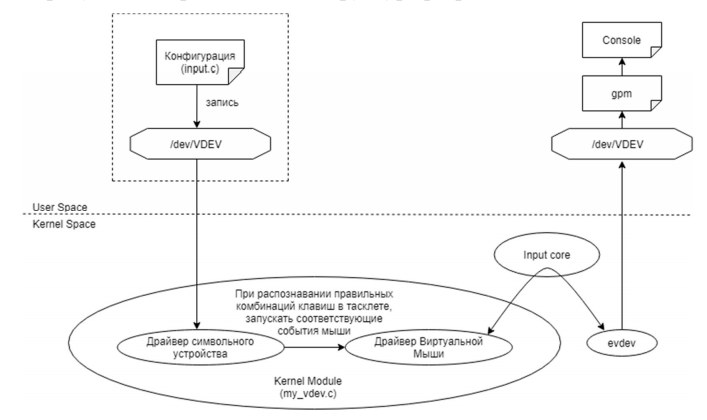
\includegraphics[width=0.7\linewidth]{src/img/module_schema}
	\caption{}
	\label{fig:moduleschema}
\end{figure}

\subsection{Основнеые структуры программы}
В этой курсовой работе символьное устройство обернуто другой структурой, называемой vdev. 
Эта структура действует на некоторую память, выделенную из ядра и содержит буфер scancode для символьного устройства. 
Она также содержит конфигурацию пользователя (листинг \ref{lst:vdev}).

\begin{lstlisting}[caption=Структура vdev, label={lst:vdev}]
static struct vdev {
	struct cdev cdev;
	spinlock_t lock;
	u8 buf[2];
	char map[8];
	int spd;
}
\end{lstlisting}

Структура struct file\_operations определяет, какие операции могут быть выполнены на символьном устройстве.
В нашем случаи символьному устройству нужно только получать конфуигурацию из пользовательского пространства, по этому реализуются только операции: открытия, закрытия, чтения (листинг \ref{lst:file_oper}).

\begin{lstlisting}[caption=Структура file\_operations, label=lst:file_oper]
static const struct file_operations vdev_fops = {
	.owner = THIS_MODULE,
	.open = vdev_open,
	.releae = vdev_release,
	.write = vdev_write,
};
\end{lstlisting}

\subsection{Формат конфигурации от пользователей}
Для обеспечения пользователей возможность настройки параметров драйвера необходимо установить формат команд. 
Команда должна состоять издвух частей:
\begin{enumerate}
	\item код команды: \begin{enumerate}
		\item 0 - настройка карты клавиатуры;
		\item 1 - настройка скорости перемещения курсора мыши.
	\end{enumerate}
	\item тело: \begin{enumerate}
		\item Если код команды 0, то тело представляет собой символьную строку состаяющую из 6 символов, обозначающих 6 клавиш, соответстующих движению вверх, вниз, влево, вправо, лкм, пкм;
		\item Если код 1, то тело представляет собой целове цисло, указывающее скорость движения мыши.
	\end{enumerate}
\end{enumerate}

\subsection{Реализация обработчика прерываний}
На рисунке \ref{fig:irqproceed} отображена реализация обработчика прерываний клавиатуры.

% TODO: \usepackage{graphicx} required
\begin{figure}[H]
	\centering
	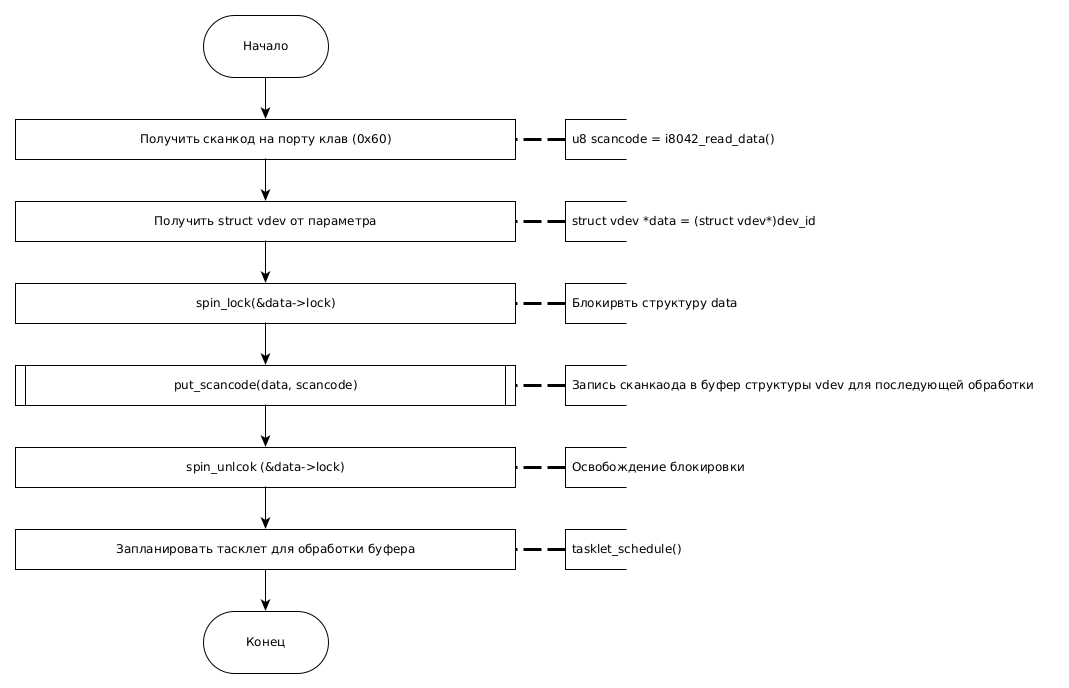
\includegraphics[width=1\linewidth]{src/img/irq_proceed}
	\caption{Реализация обработчика прерываний квалиатуры}
	\label{fig:irqproceed}
\end{figure}
